\documentclass[12pt]{article}
\usepackage{graphicx}

\begin{document}

\begin{titlepage}
\begin{center}

\includegraphics[scale=1]{Diagrams/up.jpg}
\bigskip
\bigskip
\bigskip
\begin{huge}
\textbf{Kum-Ladi}
	
\bigskip
\bigskip
\bigskip
\textbf{Buzz Discussion Forum}
\bigskip
\bigskip
\bigskip
\end{huge}

 \begin{huge}
 \textbf{Requirements and Design Specifications}
\end{huge}

\bigskip
\bigskip
\bigskip

Compiled By \\[\baselineskip]
{\large

Nkosinathi Mothoa - u12077420\\
Nkosenhle Ncube - u13247914\\
Nathan Ngobale - u15110045\\
Kamogelo Tsipa - u13010931\\
\par}

\end{center}

\end{titlepage}

\newpage
\tableofcontents

\newpage
\section{Vision and Scope}    

\subsection{Project Vision} 

\paragraph{Buzz is aimed at finding ways to enhance teaching and improve the learning of students through the use of online discussion. Through the system, there will be formations of collaborative communities within student groups, which is essential to enhance education. The forum will allow students to express their views and explore what they are learning, this will result in creating a collaborative community in which students can excel.}
\paragraph{The Buzz project also aims to create an online space where students, teaching assistants and lecturers can engage in activities related to learning the content of our module while applying game concepts to motivate students to increase the quality of their participation and consequently experience deeper learning of the course.}

\subsection{Architecture Design of Buzz System}
\paragraph{At the highest level of granularity the Buzz system is based on Service Oriented Architecture(SOA). Second level of granularity can be visualized as to be based on model-view controller.}
\paragraph{On a high-level view, the system must be an Online Transcation Processing system. This system will be most beneficial because it will allow the users to receive near instant responses to their requests. It can accommodate multiple concurrent users at the same time. The system will be able to handle all kinds of processes (mainly CRUD operations).}

\newpage
\subsubsection*{Architecture Design}
\begin{itemize}
\item Micro services
\item Model-view-control architecture patterns
\item Layered architecture patterns
\end{itemize}
\subsubsection*{Quality Requirements}
\paragraph*{The quality requirements of the Buzz system will be, but not limited to:}
\begin{itemize}
\item Security
\item Performance
\item Accessibility
\item Integrability
\item Maintainability
\item Reliability
\item Availability
\end{itemize}
\subsection{Project Scope}
\paragraph{.The core of the system is an online discussion board which applies game concepts. A basic Use case diagram of the system is show below.}

\begin{figure}[h!]
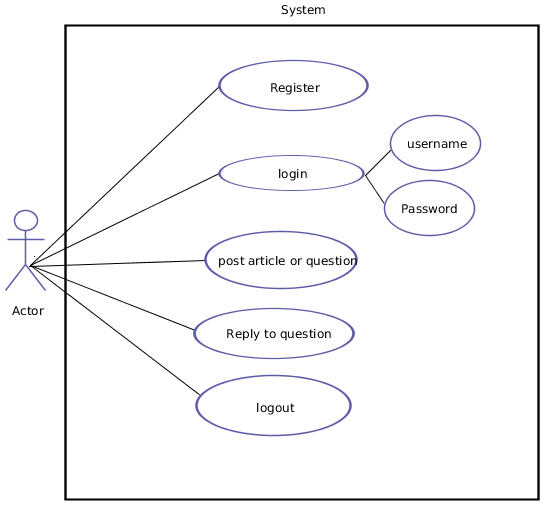
\includegraphics[scale=0.7]{Diagrams/basic_system.png}
\caption{Use case Diagram of the Buzz system.}
\end{figure}


\newpage
\subsection{Design Requirement}
\paragraph{}

\section{Application requirements and design}
\begin{itemize}
\item Users must be able to create,read,update and delete (CRUD) posts. certain users will be granted power to CRUD other user's posts in a highly controlled fashion.
\item Keep track of who has read what and highlight unread messages for each user.
\item Restrict the length of messages and the type of content allowed in messages based on the level where it is posted as well as on the status of the user posting the message.
\item Restrict users to post on specified levels based on their status of the user posting the message.
\item Allow staff to manage content i.e summaries,close or hide threads and move things around.
\item Provide functionality to support semi-automatic creation of thread summaries.
\item Create automated template based messages to individual users or specified groups.
\item Automatically change the status of a user based on participation.
\item Integrate seamlessly with any host site.
\item Provide functions such as searching and filtering.
\item Provide functionality to evaluate posts and vote for posts.
\item Use evaluation to create statistical information such as average mark of each student within a given time range. Visual reporting of a participants evaluation in relation to the average of the evaluation of all the users of a certain groups of users is required for the gratification concept.
\item Enhancement of the post editor for example text formatting and automatic pretty-printing of code in posts.
\item Provide functions to apply social tagging. Allow users to view content based on personal structure according to their own tags or according to the administration's  structure and share their tags.
\item Apply self-organization based on social tagging and allow the user to  view according to the base structure, owns structure or public structure.
\item Detect if a post is plagiarized.
\item Detect violation of etiquette rules.
\end{itemize}

\newpage

\subsection{Users Module}
\par{The user management module is responsible for maintaining information about registered users of the system. This includes different levels of authority and restrictions for each user. The Administrator can manage and control the content of posts whilst the tutors/TA's can manage the content and the violation of etiquette rules. Users who have logged in my requests services to persist content from various modules based on their needs.}
\subsubsection{Scope}
\par{The scope of the Buzz-Users Module is modeled by Figure 20. Users with the appropriate privilege will be able to perform said tasks on the Forum. All other non-admin users will be able to perform all standard forum tasks.}

\begin{figure}[h]
\iffalse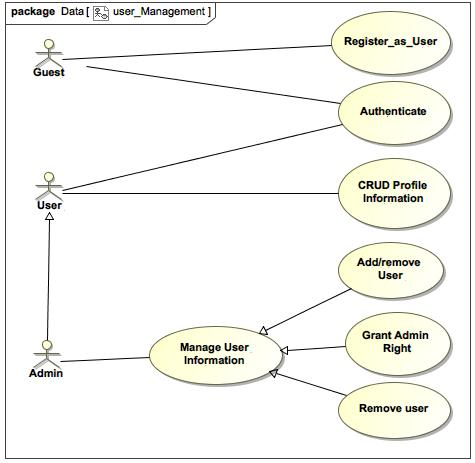
\includegraphics[scale=1]{Diagrams/scopeUsers.jpeg}\fi
\caption{Scope of the Buzz-Users Module.}
\label{Use-case: Buzz-Users Module}
\end{figure}

\subsubsection{Use cases}
\subsubsection{Service contracts}
\subsubsection{Functional Req's}
\subsubsection{Domain Model}

\subsubsection{Service contracts}

\subsubsection{Technologies}
\par{ To address the need for a loosely coupled and high cohesion system, a micro service architecture will be used. }

\begin{itemize} 
\item  REST Proxy, which is an open source HTTP-based proxy for Kafka cluster, 
\end{itemize}

\subsection{CS-Status Module}
\par{Intro to Module}
\subsubsection{Scope}
\par{The scope of the Buzz CS-Status module is modeled by Figure 45. Users CS-Status will determine the extent of their privilege on the Forum.}

\begin{figure}[h]
\iffalse\includegraphics[scale=1]{Diagrams/scopeStatus.jpeg}\fi
\caption{Scope of the Buzz-Status Module.}
\label{Use-case: Buzz-Status Module}
\end{figure}

\subsubsection{Use cases}
\subsubsection{Service contracts}
\subsubsection{Functional Req's}
\subsubsection{Domain Model}


\subsection{Notifications Module}
\par{This module will be responsible for the handling of User notifications.}
\subsubsection{Scope}
\par{The scope of the Notifications module is modeled by Figure 23. Users will have the option of subscribing to Forum content and receiving Notifications on this specific content via email}

\begin{figure}[h]
\iffalse\includegraphics[scale=1]{Diagrams/scopeNotif.jpeg}\fi
\caption{Scope of the Buzz-Notifications Module.}
\label{Use-case: Buzz-Notif Module}
\end{figure}

\subsubsection{Use cases}

\subsubsection{Service Contracts}
\paragraph{The notification requests will need to be of a specific type and properly validated before being processed. The request will fail if does not meet its specified prerequisites. In order for a notification request to be passed on to the server, the user needs to already exist on the database. if this requirement is not met, a notification request will fail.}
\begin{itemize}
\item Notify user after posting
\item Notify user of a posting
\item Remove posted notification 
\item Read posted notification
\end{itemize}

\subsubsection{Technologies}

\begin{itemize}
\item Apache Kafka will be used for data streaming of the notifications. This will allow the user's page to be updated as the information changes in the background, without the user having to refresh their page to check if any changes have been made.
\item The linking of the notification with the thread or post it is associated with will be done using JavaScript.This will allow for dynamic posting of notifications, without the administrator having to manually create every notification.
\item Google Email is an API with a capacity to service a number of email within a limit. The API will be ideal to provide messaging capacity for the system without having to implement email servers internally.
\end{itemize}

\subsubsection{Domain Model}
\par{}

\newpage
\subsection{Threads/Posts Module}
\paragraph{Intro to Module}
\subsubsection{Scope}
\subsubsection{Use cases}
\subsubsection{Service contracts}
\subsubsection{Functional Req's}
\subsubsection{Domain Model}

\paragraph{This module will model the functionality involved with the posting of messages/comments/feedback on the forum.}

\subsubsection{Requirements}
\subsubsection*{Functional}
\begin{itemize}
\item Handle the posting and accessing of forum content asd well as structuring forum threads in an orderly manner.
\item User friendly and accurate
\end{itemize}
\subsubsection*{Non-functional}
\begin{itemize}
\item User friendly and accurate
\item The notification should be able to direct the user to the appropriate thread or posted
\item Allow for an expansion of a p
\end{itemize}
\subsection*{}

\subsubsection{Use Case: Post}

\begin{itemize}
\item Each user will be able to make posts about the current topic they are in. The posts will be seen on the Internet forum message board, which enables them to participate in the discussion within the current topic / thread. The effectiveness of this is that every user is able to engage on their own free will and unlike group chats on what’s app people would be able to give url links, images, code snippet suggestions, and also other valuable information that may help with their understanding and development in the current thread.
\end{itemize}

\subsubsection{Use Case: CRUD}

\begin{itemize}
\item All users (admin and non-admin) will be able to create their own threads and posts but non-admin users will be able to delete their posts based on certain restrictions , example if they had made a post or a thread that has not been given any comment or follow up post, the create will be able to delete it incase they feel it will useless.
Non-admin users will be restricted as to the things they, will not be able to delete other peoples posts. Administrators will be able to delete posts also viewing statistics on individual users.
\end{itemize}

\subsection{Buzz Forum-Modules Module}
\par{The Buzz Forum-Modules module models the course spaces of the forum and separates forum topics into their respective course mudules (ie: COS 121 and COS 212 will have their own Buzz Forum-Module)}
\subsubsection{Scope}
\par{The scope of the Buzz-Subscriptions Module is modeled by Figure 22. Users with the appropriate privilege will be able to CRUD and manage Forum-Modules}

\begin{figure}[h]
\iffalse\includegraphics[scale=1]{Diagrams/scopeForumModules.jpeg}\fi
\caption{Scope of the Buzz-ForumModule Module.}
\label{Use-case: Buzz-ForumModules}
\end{figure}

\subsubsection{Use cases}
\subsubsection{Service contracts}
\subsubsection{Functional Req's}
\subsubsection{Domain Model}

\subsection{Authorization Module}
\par{}
\subsubsection{Scope}
\par{}

\begin{figure}[h]
\iffalse\includegraphics[scale=1]{Diagrams/scopeAuth.jpeg}\fi
\caption{Scope of the Buzz-Authorization Module.}
\label{Use-case: Buzz-Auth}
\end{figure}

\subsubsection{Use cases}
\subsubsection{Service contracts}
\subsubsection{Functional Req's}
\subsubsection{Domain Model}

\subsection{Data-Sources Module}
\par{Intro to Module}
\subsubsection{Scope}
\par{}

\begin{figure}[h]
\iffalse\includegraphics[scale=1]{Diagrams/scopeDataSources.jpeg}\fi
\caption{Scope of the Buzz-DataSources Module.}
\label{Use-case: Buzz-Data Sources}
\end{figure}

\subsubsection{Use cases}
\subsubsection{Service contracts}
\subsubsection{Functional Req's}
\subsubsection{Domain Model}

\subsection{Reporting and Data Module}
\par{Intro to Module}
\subsubsection{Scope}
\par{}

\begin{figure}[h]
\iffalse\includegraphics[scale=1]{Diagrams/scopeRaD.jpeg}\fi
\caption{Scope of the Buzz Reports and Data Module.}
\label{Use-case: Buzz-Reports and Data}
\end{figure}

\subsubsection{Use cases}
\subsubsection{Service contracts}
\subsubsection{Functional Req's}
\subsubsection{Domain Model}

\subsection{Web Module}
\par{Intro}
\subsubsection{Scope}
\par{}

\begin{figure}[h]
\iffalse\includegraphics[scale=1]{Diagrams/scopeWeb.jpeg}\fi
\caption{Scope of the Buzz-Web Module.}
\label{Use-case: Buzz-Web}
\end{figure}

\subsubsection{Use cases}
\subsubsection{Service contracts}
\subsubsection{Functional Req's}
\subsubsection{Domain Model}

\subsection{Buzz-Gamification Module}
\par{Intro to Module}
\subsubsection{Scope}
\par{}

\begin{figure}[h]
\iffalse\includegraphics[scale=1]{Diagrams/scopeGamification.jpeg}\fi
\caption{Scope of the Buzz-Gamification Module.}
\label{Use-case: Buzz-Gamification}
\end{figure}

\subsubsection{Use cases}
\subsubsection{Service contracts}
\subsubsection{Functional Req's}
\subsubsection{Domain Model}

\subsection{Buzz-Subscriptions Module}
\par{The Buzz-Subscriptions module handles content subscriptions made by the user. These include subscriptions to Posts and/or forum topics.}
\subsubsection{Scope}
\par{The scope of the Buzz-Subscriptions Module is modeled by Figure 25. Users have the option of subscribing to particular Posts or Forum topics. The User will then have the option to receive Notifications via email on the content of their subscriptions.}

\begin{figure}[h]
\iffalse\includegraphics[scale=1]{Diagrams/scopeSubscriptions.jpeg}\fi
\caption{Scope of the Buzz-Subscriptions Module.}
\label{Use-case: Buzz-Subscriptions}
\end{figure}

\subsubsection{Use cases}
\subsubsection{Service contracts}
\subsubsection{Functional Req's}
\subsubsection{Domain Model}

\end{document}
